\chapter[Deep water formation]{Transport of microbial cells during deep water formation}
\label{ch:deepwaterformation}

\section{Abstract}

During sampling for the study presented in \secreft{ch:polarfront}, additional samples were collected of \ac{AABW} on the Antarctic continental shelf and from the sea floor in the vicinity of the mid-ocean ridge.
Metagenomic analysis found that the community composition of the continental shelf samples was surprisingly similar to that of surface samples in the same area, despite the significant differences in environmental factors such as pressure and light availability.
This may have resulted from the rapid advection of cells in the sinking of surface waters to form \ac{AABW} (deep water formation; see \secreft{ch:intro}).
These results led to the study described in \secreft{ch:advection}.

\glsresetall

\section{Introduction}

The Mertz Glacier polynya is a region of open ocean (bound by the Antarctic coast, sea ice and the Mertz glacier tongue) west of the Mertz Glacier tongue (approx. 67\textdegree{} S, 145\textdegree{} E).
The polynya has historically been a major site for the formation of \ac{AABW} in the \ac{SO}, although its role in this process has become less clear following the calving of a large section of the glacier tongue in February 2010 \cite{Tamura:2012da}.
Evaporative cooling of the sea surface by katabatic winds from the Antarctic continent, combined with the exclusion of salt from forming sea ice (``brine exclusion'' or ``brine rejection''), results in the rapid formation and sinking of cold, dense water \cite{Williams:2008iu}.
This water forms an abyssal layer in the Ad\'{e}lie depression (a bathymetric feature underlying the polynya), eventually outflowing northwards over the continental sill as part of the \ac{AABW}.

This brief chapter presents an exploratory analysis of two abyssal samples of \ac{AABW} from within the Ad\'{e}lie depression, and one from the South Australian basin further north.
The results from this study led to the investigation of advective transport of microorganisms described in \secreft{ch:advection}.

\section{Methods}

\begin{table}
\sffamily
\footnotesize
\caption[\ac{AABW} samples used in the preliminary analysis]{Sampling time, location and physicochemical properties of \ac{AABW} samples used in this preliminary study.
All data were retrieved from the \ac{CTD} (SeaBird, Bellevue, USA) instrument used to collect the samples.}
\label{tab:deepsamples}
\begin{tabu} to\textwidth{llllIZXX}
\toprule
\textbf{Sample} & \textbf{Date} & \textbf{Latitude} & \textbf{Longitude} & \textbf{Depth (m)} & \textbf{Temperature (\textdegree{}C)} & \textbf{Salinity (PSU)} & \textbf{Volume \linebreak filtered (L)}\\
\midrule
356 & 03/01/2008 & \textminus{}66.76 & 144.41 & 920 & -1.9 & 34.69 & 230\\
361 & 14/01/2008 & \textminus{}66.47 & 140.56 & 1170 & -1.8 & 34.56 & 225\\
365 & 23/01/2008 & \textminus{}56.70 & 141.91 & 3693 & 0.5 & 34.69 & 230\\
\bottomrule
\end{tabu}
\end{table}

% the sample map
\begin{figure}
  \centering
  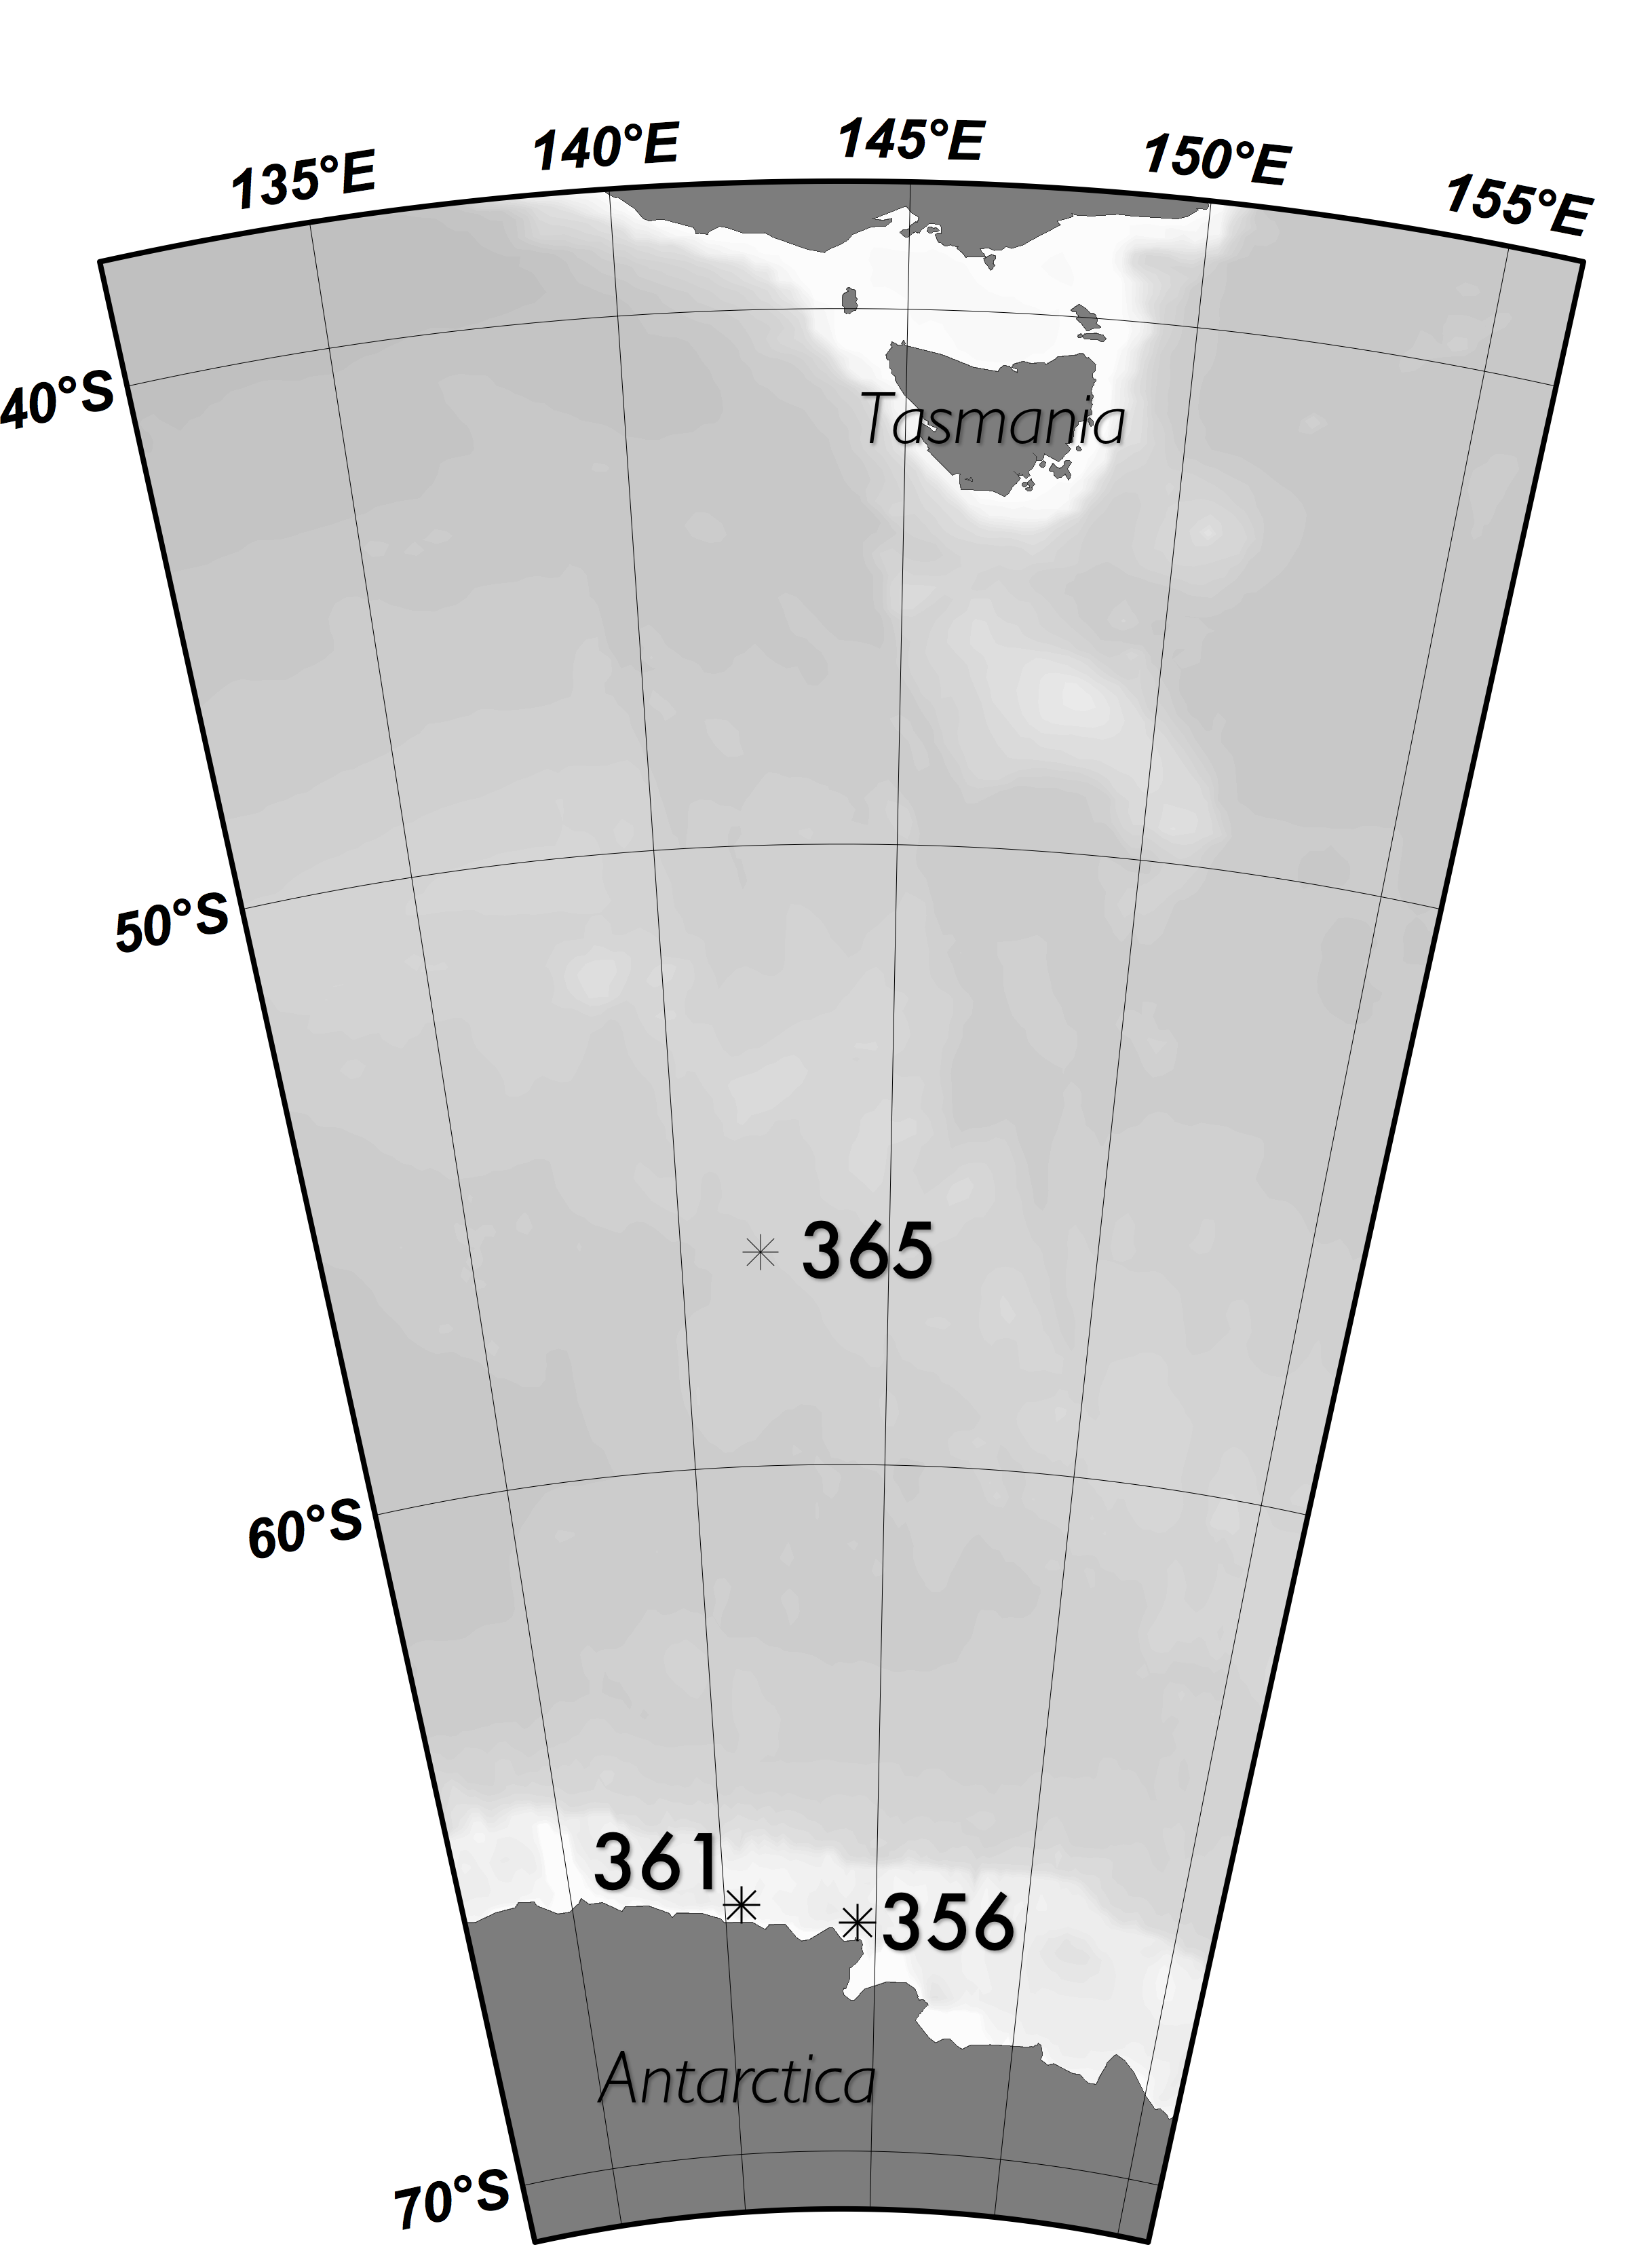
\includegraphics[width=\textwidth]{../deepwaterformation/deepsamplemap.png}
  \caption[Map showing sites of preliminary \ac{AABW} samples]{Sites of preliminary \ac{AABW} samples.}
  \label{fig:deepsamplemap}
\end{figure}


Three samples of \ac{AABW} were opportunistically obtained and analysed during the project described in \secreft{ch:polarfront} \figref{fig:deepsamplemap}.
Two of these samples (356 and 361) were of newly formed \ac{AABW} waters on the Antarctic continental shelf, while one (365) was of abyssal \ac{AABW} from the South Australian basin \tabref{tab:deepsamples}.
DNA extraction, sequencing and construction of a taxonomic profile by \softwarename{blast} comparison to the RefSeq database and processing with \ac{GAAS} were performed using the methods described in \secreft{ch:polarfront}.
A standardised and log-transformed Bray-Curtis resemblance matrix was constructed including the taxonomic profiles of the \ac{AABW} samples as well as the \ac{NZ} and \ac{SZ} samples described in \secreft{ch:polarfront}.
A \ac{nMDS} plot was then constructed from this matrix.
All statistical procedures were performed in \softwarename{PRIMER 6} as described by \citet{Clarke:2001ut}.

\section{Results and Discussion}

Although the three \ac{AABW} samples were taken in deep, cold and aphotic waters \tabref{tab:deepsamples} compared to the surface \ac{AZ} and \ac{SZ} samples, the \ac{nMDS} plot suggested that the two continental shelf \ac{AABW} samples (356 and 361) were surprisingly similar to those of the \ac{AZ}, particularly sample 353 \figref{fig:deepnmds}.
Further, the indicated the presence of several \acp{OTU} which would not be expected to be present at significant abundance in deep, aphotic waters \tabref{tab:topdeepotus}.
For example, \species{Roseobacter denitrificans} OCh 114, a model organism for aerobic anoxygenic photosynthesis, was the fifth most abundant \ac{OTU} of the continental shelf samples.
Numerous \ac{CFB} representatives, typically associated with \ac{POM} and the utilisation of \ac{HMW} phytoplankton products \citep[e.g.][]{Williams:2012gsa}, were also unexpectedly high.

\begin{landscape}
\begin{table}
\centering
\sffamily
\caption[Twenty most abundant \acp{OTU} in preliminary \ac{AABW} samples]{Relative abundances (as percentages) of the twenty most abundant \acp{OTU} identified in the preliminary study of \ac{AABW} samples.}
\label{tab:topdeepotus}
\begin{tabular}{lS[table-format=2.5]S[table-format=2.5]S[table-format=2.5]S[table-format=2.5]S[table-format=2.5]S[table-format=2.5]}
\toprule
\textbf{OTU} & \multicolumn{3}{c}{\textbf{Sample 356}} & \multicolumn{3}{c}{\textbf{Sample 365}}\\
\cmidrule(r){2-4}
\cmidrule(r){5-7}
& {0.1 \micron} & {0.8 \micron} & {3.0 \micron} & {0.1 \micron} & {0.8 \micron} & {3.0 \micron}\\
\midrule
\candidatusfull{Pelagibacter ubique} HTCC1062 & 48.40 & 32.32 & 32.85 & 19.02 & 22.31 & 3.880\\
\speciesfull{Nitrosopumilus maritimus} SCM1 & 11.92 & 9.289 & 13.99 & 30.17 & 7.790 & 22.74\\
\candidatusfull{Ruthia magnifica} str. Cm (\species{Calyptogena magnifica}) & 3.780 & 4.563 & 2.356 & 2.844 & 1.504 & 0.2599\\
\candidatusfull{Vesicomyosocius okutanii} strain HA & 2.349 & 2.757 & 1.396 & 1.859 & 0.8025 & 0.08227\\
\genus{Roseobacter} sp. OCh 114 & 0.1412 & 1.166 & 0.6845 & 0.08564 & 0.6662 & 0.4851\\
\candidatusfull{Puniceispirillum marinum} IMCC1322 & 0.3180 & 1.103 & 0.6403 & 0.4218 & 0.8223 & 0.4202\\
\species{Marinobacter hydrocarbonoclasticus} VT8 & 0.06999 & 0.4091 & 0.3976 & 0.2476 & 1.050 & 2.338\\
\species{Silicibacter pomeroyi} DSS-3 & 0.1081 & 0.8406 & 0.4996 & 0.1290 & 0.4630 & 0.3621\\
\species{Robiginitalea biformata} strain HTCC2501 & 0.2813 & 0.6433 & 0.7417 & 0.1769 & 0.2739 & 0.4978\\
\species{Pseudoalteromonas haloplanktis} strain TAC125 & 0.02530 & 0.4540 & 0.1958 & 0.2836 & 2.817 & 0\\
\species{Alcanivorax borkumensis} strain SK2 & 0.09262 & 0.3163 & 0.4281 & 0.1049 & 0.5674 & 1.985\\
\species{Gramella forsetii} strain KT0803 & 0.3096 & 0.6465 & 0.7405 & 0.1254 & 0.2670 & 0\\
\genus{Colwellia} sp. 34H & 0.04289 & 0.4512 & 1.020 & 0.07200 & 0.4532 & 0.7727\\
\species{Flavobacterium psychrophilum} strain JIP02/86 & 0.2417 & 0.4722 & 0.6353 & 0.07943 & 0.1645 & 0.5072\\
\species{Pirellula staleyi} strain DSM 6068 & 0.003149 & 0.2477 & 0.3093 & 0.08767 & 1.401 & 0.7732\\
\genus{Jannaschia} sp. DFL-12 & 0.07995 & 0.6770 & 0.3841 & 0.03865 & 0.2030 & 0.1025\\
\species{Pseudoalteromonas atlantica} strain T6c & 0.02312 & 0.1653 & 0.1941 & 0.03856 & 0.3235 & 1.728\\
\species{Zunongwangia profunda} strain SM-A87 & 0.1830 & 0.3499 & 0.4826 & 0.1036 & 0.1362 & 0.3825\\
\genus{Silicibacter} sp. TM1040 & 0.09568 & 0.5448 & 0.3455 & 0.03477 & 0.2014 & 0.1740\\
\species{Capnocytophaga ochracea} strain DSM 7271 & 0.1251 & 0.2916 & 0.4491 & 0.03893 & 0.1542 & 0.5332\\
\bottomrule
\end{tabular}
\end{table}
\end{landscape}


A possible explanation for these observations is that the continental shelf samples represent \ac{AABW} recently formed in the D'Urville sea, and the observed assemblage therefore represents advection rather than selection by environmental factors.
The project described in \secreft{ch:advection} was designed to test and explore this hypothesis.

\begin{figure}[!ht]
  \centering
  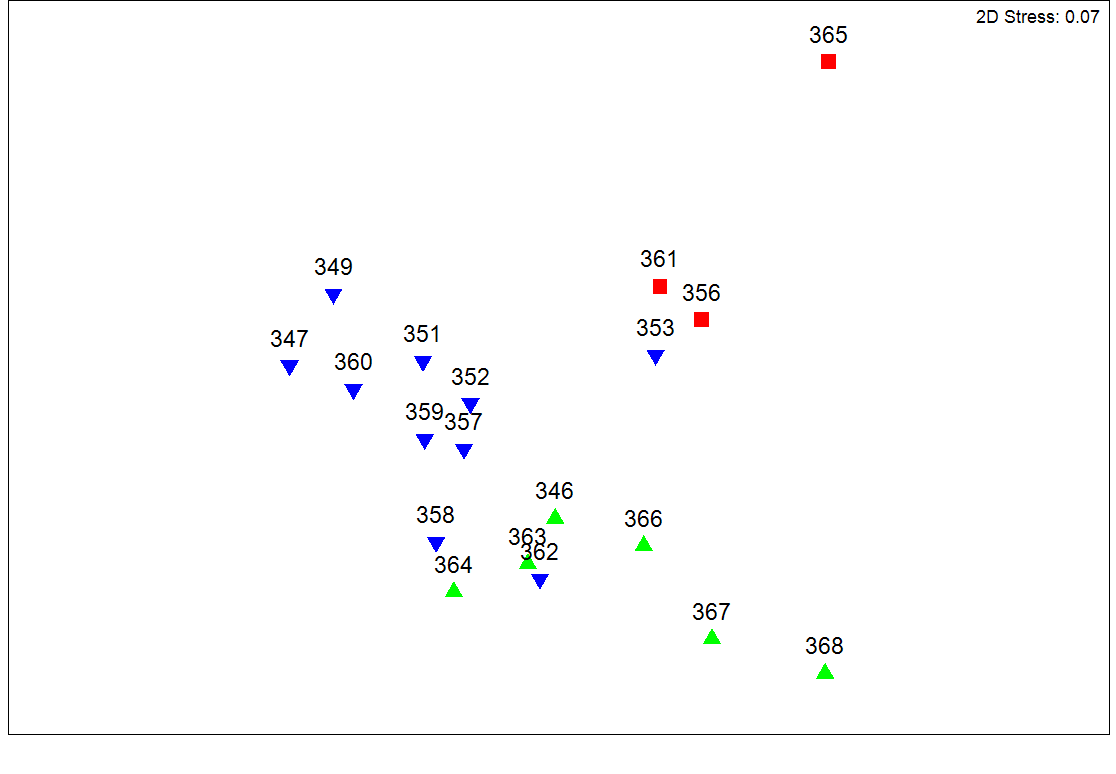
\includegraphics[width=\textwidth]{../deepwaterformation/deepnmds.png}
  \caption[\ac{nMDS} of \ac{AABW}, \ac{NZ} and \ac{SZ} samples]{\ac{nMDS} plot showing distance between \ac{AABW}, \ac{NZ} and \ac{SZ} samples.
  Green triangles represent samples from the \ac{NZ}; blue inverted triangles from the \ac{SZ}; and red squares from \ac{AABW}.}
  \label{fig:deepnmds}
\end{figure}

